\documentclass[11pt,openany]{article}

\usepackage{mathtools, commath}
% Packages for formatting
\usepackage[margin=1in]{geometry}
\usepackage{fancyhdr}
\usepackage{enumerate}
\usepackage{graphicx}
\usepackage{kotex}
\usepackage{arydshln} % Include this package
\usepackage{bbding}
\usepackage{amsmath}
\usepackage{amsthm}
\usepackage[dvipsnames,table]{xcolor}
\usepackage{amssymb, amsfonts}
\usepackage{wasysym}
\usepackage{footnote}
\usepackage{tablefootnote}
\usepackage{arydshln} % Include this package
\usepackage{framed}
\usepackage{physics}

% Fonts
\usepackage[T1]{fontenc}
\usepackage[utf8]{inputenc}
\usepackage{newpxtext,newpxmath}
\usepackage{sectsty}

% Define colors
\definecolor{TealBlue1}{HTML}{0077c2}
\definecolor{TealBlue2}{HTML}{00a5e6}
\definecolor{TealBlue3}{HTML}{b3e0ff}
\definecolor{TealBlue4}{HTML}{00293c}
\definecolor{TealBlue5}{HTML}{e6f7ff}

\definecolor{thmcolor}{RGB}{231, 76, 60}
\definecolor{defcolor}{RGB}{52, 152, 219}
\definecolor{lemcolor}{RGB}{155, 89, 182}
\definecolor{corcolor}{RGB}{46, 204, 113}
\definecolor{procolor}{RGB}{241, 196, 15}

\usepackage{color,soul}
\usepackage{soul}
\newcommand{\mathcolorbox}[2]{\colorbox{#1}{$\displaystyle #2$}}
\usepackage{cancel}
\newcommand\crossout[3][black]{\renewcommand\CancelColor{\color{#1}}\cancelto{#2}{#3}}
\newcommand\ncrossout[2][black]{\renewcommand\CancelColor{\color{#1}}\cancel{#2}}

\usepackage{hyperref}
\usepackage{booktabs}

% Chapter formatting
\definecolor{titleTealBlue}{RGB}{0,53,128}
\usepackage{titlesec}
\titleformat{\section}
{\normalfont\sffamily\LARGE\bfseries\color{titleTealBlue!100!gray}}{\thesection}{1em}{}
\titleformat{\subsection}
{\normalfont\sffamily\Large\bfseries\color{titleTealBlue!85!gray}}{\thesubsection}{1em}{}
\titleformat{\subsubsection}
{\normalfont\sffamily\Large\bfseries\color{titleTealBlue!70!gray}}{\thesubsubsection}{1em}{}

%Tcolorbox
\usepackage[most]{tcolorbox}
\usepackage{multirow}
\usepackage{multicol}
\usepackage{blindtext}

\usepackage[linesnumbered,ruled]{algorithm2e}
\usepackage{algpseudocode}
\usepackage{setspace}
\SetKwComment{Comment}{/* }{ */}
\SetKwProg{Fn}{Function}{:}{end}
\SetKw{End}{end}
\SetKw{DownTo}{downto}

% Define a new environment for algorithms without line numbers
\newenvironment{algorithm2}[1][]{
	% Save the current state of the algorithm counter
	\newcounter{tempCounter}
	\setcounter{tempCounter}{\value{algocf}}
	% redefine the algorithm numbering (remove prefix)
	\renewcommand{\thealgocf}{}
	\begin{algorithm}
	}{
	\end{algorithm}
	% Restore the algorithm counter state
	\setcounter{algocf}{\value{tempCounter}}
}

\usepackage{adjustbox}
% Header and footer formatting
\pagestyle{fancy}
\fancyhead{}
\fancyhf{}
\rhead{\textcolor{TealBlue2}{\large\textbf{리만의 복소해석을 토대로 얻는 내 수학적 시야 (2기)}}}%\rule{3cm}{0.4pt}}
\lhead{\textcolor{TealBlue2}{\large\textbf{수학의 즐거움, Enjoying Math}}}
% Define footer
%\newcommand{\footer}[1]{
%\begin{flushright}
%	\vspace{2em}
%	\includegraphics[width=2.5cm]{school_logo.jpg} \\
%	\vspace{1em}
%	\textcolor{TealBlue2}{\small\textbf{#1}}
%\end{flushright}
%}
%\rfoot{\large Department of Information Security, Cryptogrphy and Mathematics, Kookmin Uni.\includegraphics[height=1.5cm]{school_logo.jpg}}
\fancyfoot{}
\fancyfoot[C]{-\thepage-}

\usepackage{animate}
% Load the PDF and grab its total pages into \NumPages:
\newcount\NumPagesA
\pdfximage{riemann-tikz/secant_line_gif.pdf}% loads the PDF
\NumPagesA=\pdflastximagepages
\usepackage{tcolorbox}
\tcbset{colback=white, arc=5pt}

\definecolor{axiomcolor}{HTML}{a88bfa}
\definecolor{defcolor}{RGB}{52, 152, 219}
\definecolor{procolor}{RGB}{241, 196, 15}
\definecolor{thmcolor}{RGB}{231, 76, 60}
\definecolor{lemcolor}{RGB}{155, 89, 182}
\definecolor{corcolor}{RGB}{46, 204, 113}
\definecolor{execolor}{RGB}{90, 128, 127}

% Define a new command for the custom tcolorbox
\newcommand{\axiombox}[2][]{%
	\begin{tcolorbox}[colframe=axiomcolor, title={\color{white}\bfseries #1}]
		#2
	\end{tcolorbox}
}

\newcommand{\defbox}[2][]{%
	\begin{tcolorbox}[colframe=defcolor, title={\color{white}\bfseries #1}]
		#2
	\end{tcolorbox}
}

\newcommand{\lembox}[2][]{%
	\begin{tcolorbox}[colframe=lemcolor, title={\color{white}\bfseries #1}]
		#2
	\end{tcolorbox}
}

\newcommand{\probox}[2][]{%
	\begin{tcolorbox}[colframe=procolor, title={\color{white}\bfseries #1}]
		#2
	\end{tcolorbox}
}

\newcommand{\thmbox}[2][]{%
	\begin{tcolorbox}[colframe=thmcolor, title={\color{white}\bfseries #1}]
		#2
	\end{tcolorbox}
}

\newcommand{\corbox}[2][]{%
	\begin{tcolorbox}[colframe=corcolor, title={\color{white}\bfseries #1}]
		#2
	\end{tcolorbox}
}



\usepackage{amsthm}

% Define custom theorem styles
\newtheoremstyle{dotless} % Name of the style
{3pt} % Space above
{3pt} % Space below
{\itshape} % Body font
{} % Indent amount
{\bfseries} % Theorem head font
{} % Punctuation after theorem head
{2.5mm} % Space after theorem head
{} % Theorem head spec

\newtheoremstyle{definitionstyle} % Name of the style
{3pt} % Space above
{3pt} % Space below
{} % Body font
{} % Indent amount
{\bfseries} % Theorem head font
{.} % Punctuation after theorem head
{2.5mm} % Space after theorem head
{} % Theorem head spec

% Applying custom styles
%\theoremstyle{dotless}
\newtheorem{theorem}{Theorem} % Theorem environment with section-wise numbering
\newtheorem*{theorem*}{Theorem} % Theorem environment with section-wise numbering
\newtheorem*{lemma*}{Lemma} % Theorem environment with section-wise numbering
\newtheorem*{proposition*}{Proposition} % Theorem environment with section-wise numbering
\newtheorem*{corollary*}{Corollary} % Theorem environment with section-wise numbering
\newtheorem{proposition}[theorem]{Proposition} % Theorem environment with section-wise numbering
\newtheorem{lemma}[theorem]{Lemma} % Lemma shares the counter with theorem
\newtheorem{corollary}[theorem]{Corollary} % Corollary shares the counter with theorem

\theoremstyle{definitionstyle}
\newtheorem*{observation}{\textcolor{Magenta}{Observation}}
\newtheorem{claim}{Claim}
\newtheorem{definition}{Definition} % Definition shares the counter with theorem
\newtheorem{example}{Example} % Example shares the counter with theorem
\newtheorem{exercise}{{Exercise}} % Example shares the counter with theorem
\newtheorem{remark}{Remark} % Remark shares the counter with theorem
\newtheorem*{note}{Note}

\newtheorem*{axiom*}{Axiom}
\newtheorem*{definition*}{Definition} % Definition shares the counter with theorem
\newtheorem*{example*}{Example} % Example shares the counter with theorem
\newtheorem*{exercise*}{\textcolor{teal}{Exercise}} % Example shares the counter with theorem
\newtheorem*{remark*}{Remark} % Remark shares the counter with theorem


\usepackage{tikz}
\usepackage{tikz-cd}
\usepackage{tikz-3dplot}
\usepackage{pgfplots}
\pgfplotsset{compat=newest} % Adjust to your version of pgfplots
\def\Circlearrowleft{\ensuremath{%
		\rotatebox[origin=c]{180}{$\circlearrowleft$}}}
\def\Circlearrowright{\ensuremath{%
		\rotatebox[origin=c]{180}{$\circlearrowright$}}}
\def\CircleArrowleft{\ensuremath{%
		\reflectbox{\rotatebox[origin=c]{180}{$\circlearrowleft$}}}}
\def\CircleArrowright{\ensuremath{%
		\reflectbox{\rotatebox[origin=c]{180}{$\circlearrowright$}}}}
\usetikzlibrary{
	3d, % For 3D drawing
	angles,
	arrows,
	arrows.meta,
	backgrounds,
	bending,
	calc,
	decorations.pathmorphing,
	decorations.pathreplacing,
	decorations.markings,
	fit,
	matrix,
	patterns,
	patterns.meta,
	positioning,
	quotes,
	shadows,
	shapes,
	shapes.geometric,
	tikzmark
}
\tikzset{
	% single mid‐path arrow
	mid arrow/.style={
		decoration={
			markings,
			mark=at position 0.5 with {\arrow{Stealth[scale=1.2]}}
		},
		postaction={decorate},
	},
	% style for field arrows
	field arrow/.style={
		-{Stealth[scale=1.0]},
		thick,
		blue!70!black,
	},
}
\newcommand{\ie}{\textnormal{i.e.}}
\newcommand{\rsa}{\mathsf{RSA}}
\newcommand{\rsacrt}{\mathsf{RSA}\textendash\mathsf{CRT}}
\newcommand{\inv}[1]{#1^{-1}}

%New Command
%\newcommand{\set}[1]{\left\{#1\right\}}
\newcommand{\N}{\mathbb{N}}
\newcommand{\Z}{\mathbb{Z}}
\newcommand{\Q}{\mathbb{Q}}
\newcommand{\R}{\mathbb{R}}
\newcommand{\cR}{\mathcal{R}}
\newcommand{\C}{\mathbb{C}}
\newcommand{\F}{\mathbb{F}}
\newcommand{\nbhd}{\mathcal{N}}
\newcommand{\Log}{\operatorname{Log}}
\newcommand{\Arg}{\operatorname{Arg}}
%\newcommand{\pv}{\operatorname{P.V.}}

\newcommand{\of}[1]{\left( #1 \right)} 
%\newcommand{\abs}[1]{\left\lvert #1 \right\rvert}
%\newcommand{\norm}[1]{\left\| #1 \right\|}

\newcommand{\sol}{\textcolor{magenta}{\bf Sol}}
\newcommand{\conjugate}[1]{\overline{#1}}

%\newcommand{\res}{\operatorname{res}}
%\DeclareMathOperator*{\Res}{\operatorname{Res}}

%\renewcommand{\Re}{\operatorname{Re}}
%\renewcommand{\Im}{\operatorname{Im}}

\newcommand{\cyclic}[1]{\langle #1 \rangle}
\newcommand{\uniform}{\overset{\$}{\leftarrow}}
\newcommand{\xmark}{\textcolor{red}{\XSolidBrush}}
\newcommand{\vmark}{\textcolor{green!75!black}{\CheckmarkBold}}

\newcommand{\gen}[1]{\langle #1 \rangle}
\newcommand{\Gen}[1]{\left\langle #1 \right\rangle}

\newcommand{\img}[1]{\text{Img}(#1)}
\newcommand{\Img}[1]{\text{Img}\left(#1\right)}
\newcommand{\preimg}[1]{\text{Img}^{-1}(#1)}
\newcommand{\Preimg}[1]{\text{Img}^{-1}\left(#1\right)}

\newcommand{\relation}{\mathrel{\mathcal{R}}}
\newcommand{\injection}{\rightarrowtail}
\newcommand{\surjection}{\twoheadrightarrow}
\newcommand{\id}{\textnormal{id}}

\newcommand{\eqclass}[1]{\left[#1\right]}

% Define custom colors for O and X
\newcommand{\yes}{\textcolor{blue}{\bf \fullmoon}}
\newcommand{\no}{\textcolor{red}{\bf \texttimes}}

\DeclarePairedDelimiter\ceil{\lceil}{\rceil}
\DeclarePairedDelimiter\floor{\lfloor}{\rfloor}
%\renewcommand{\floor}[#1]{\lfloor #1\rfloor}
%\newcommand{\Floor}[#1]{\left\lfloor #1\right\rfloor}
%\newcommand{\ceil}[#1]{\lceil #1\rceil}
%\newcommand{\Ceil}[#1]{\left\lceil #1\right\rceil}

\newcommand{\topology}{\mathscr{T}}
\newcommand{\sequence}[1]{\langle #1\rangle}

% Topology
%\newcommand{\nbhd}{\mathcal{N}}

% Linear Algebra
\newcommand{\Span}{\operatorname{\normalfont span}}
\newcommand{\basis}{\mathcal{B}}
\newcommand{\card}[1]{\text{\normalfont card}(#1)}
\renewcommand{\vec}[1]{\mathbf{#1}}
\renewcommand{\emph}[1]{\textbf{#1}}
\renewcommand{\d}{\mathrm{d}} % For the exterior derivative 'd'
\newcommand{\pderiv}[2]{\frac{\partial #1}{\partial #2}}
\newcommand{\spderiv}[3]{\frac{\partial^2 #1}{\partial #2\partial #3}}
\newcommand{\vect}[1]{\begin{bmatrix} #1 \end{bmatrix}}
\newcommand{\ord}{\operatorname{ord}}

\usepackage{esvect}
\usepackage{physics}
\setstretch{1.25}

\definecolor{titleblue}{RGB}{22,72,130}
\definecolor{softgray}{RGB}{245,247,250}
\definecolor{rulegray}{RGB}{210,215,222}
\definecolor{noteblue}{RGB}{232,241,252}
\definecolor{warnred}{RGB}{252,237,237}
\definecolor{greenbox}{RGB}{236,247,238}

\newenvironment{infobox}{%
	\def\FrameCommand{\fboxrule=0.8pt \fboxsep=8pt \colorbox{noteblue}}%
	\MakeFramed{\advance\hsize-\width \FrameRestore}}{\endMakeFramed}

\newenvironment{warningbox}{%
	\def\FrameCommand{\fboxrule=0.8pt \fboxsep=8pt \colorbox{warnred}}%
	\MakeFramed{\advance\hsize-\width \FrameRestore}}{\endMakeFramed}

\newenvironment{greenboxenv}{%
	\def\FrameCommand{\fboxrule=0.8pt \fboxsep=8pt \colorbox{greenbox}}%
	\MakeFramed{\advance\hsize-\width \FrameRestore}}{\endMakeFramed}

\newcommand{\CP}{\mathbb{CP}}
\newcommand{\PP}{\mathbb{P}}
\newcommand{\OO}{\mathcal{O}}
\newcommand{\MM}{\mathcal{M}}
\newcommand{\Div}{\operatorname{Div}}
\newcommand{\Pic}{\operatorname{Pic}}
%\newcommand{\ord}{\operatorname{ord}}
\newcommand{\Hom}{\operatorname{Hom}}
\newcommand{\im}{\operatorname{im}}
\newcommand{\rk}{\operatorname{rk}}
\newcommand{\Spec}{\operatorname{Spec}}
\newcommand{\degd}{\operatorname{deg}}
\newcommand{\ellD}{\ell}
\newcommand{\CPone}{\CP^1}
\newcommand{\into}{\hookrightarrow}
\newcommand{\surj}{\twoheadrightarrow}

\renewcommand{\div}{\operatorname{div}}
\newcommand{\Prin}{\operatorname{Prin}}

\begin{document}
\pagenumbering{arabic}
\begin{center}
	\Huge\textbf{Riemann-Roch Theorem on $\C\mathbb P^1$}\\
	\vspace{0.5em}
	\large{Ji, Yonghyeon}\\
	\vspace{0.5em}
	\normalsize{\today}\\
\end{center} 
\noindent 
We cover the following topics in this note.
\begin{itemize}
	\item Complex Projective Line $\CPone$
	\item (Principal) Divisors on $\CPone$
	\item Riemann-Roch Space $L(D)$
	\item TBA
\end{itemize}

\medskip

\begin{infobox}
%The goal of this note is to understand the Riemann--Roch theorem in the nontrivial compact Riemann surface, namely \[
%X=\CPone.
%\]
On a general compact Riemann surface $X$, \textbf{Riemann--Roch} says
\[
\ell(D)-\ell(K-D)=\degd D+1-g,
\]
where
\begin{itemize}
	\item $D$ is a divisor,
	\item $K$ is a canonical divisor,
	\item $g$ is the genus,
	\item $\ell(D)=\dim_{\C} L(D)$, where
	\[
	L(D):=\{f\in \MM(X): (f)+D\ge 0\}\cup\{0\}.
	\]
\end{itemize}
For $X=\CPone$ we have $g=0$, so the theorem becomes
\[
\ell(D)-\ell(K-D)=\degd D+1.
\]
The key observation on $\CPone$ is that every divisor is linearly equivalent to a multiple of $[\infty]$: \[
D\sim(\deg D)\cdot[\infty].
\]
%, so the entire theorem reduces to explicit calculations with rational functions and polynomials.
\end{infobox}
\newpage
\tableofcontents
\subsection*{Notation}
\begin{itemize}
	\item[$\OO(X)$] Field of holomorphic functions on $X$
	\item[$\OO(X)^\times$] Field of holomorphic functions on $X$ except vanishing function
	\item[$\MM(X)$] Field of meromorphic functions on $X$
	\item[$\MM(X)^\times$] Field of meromorphic functions on $X$ except zero function
	\item[$\OO_X^\times$] Sheaf of holomorphic functions on $X$
	\item[$\MM_X^\times$] Sheaf of meromorphic functions on $X$
	\item[$L(D)$] The vector space of meromorphic functions whose poles are bounded by $D$
	\item[$\ell(D)$] $\dim_{\C}L(D)$
\end{itemize}
%\begin{description}
%	\item[$\MM(X)$] Field of meromorphic functions on $X$
%	\item[$\MM(X)^\times$] Field of meromorphic functions on $X$ except zero function
%	\item[$\MM_X^\times$] Sheaf of meromorphic functions on $X$
%\end{description}

\newpage
\section{Coordinates on $\CPone$}
\defbox[Complex Projective Line]{\begin{definition}
	The \textbf{complex projective line} is the quotient \[
	\CPone=(\C^2\setminus\{(0,0)\})/\sim,
	\] where \[
	(Z_0,Z_1)\sim(Z_0',Z_1')\iff (Z_0,Z_1)=(\lambda Z_0',\lambda Z_1')
	\] for some $\lambda\in\C^\times$.
	The class of $(Z_0,Z_1)$ is denoted by $[Z_0:Z_1]$.
\end{definition}}
\begin{remark}
The two standard affine charts are
\[
U_0=\{[Z_0:Z_1]\in\CPone: Z_0\neq 0\},
\qquad
U_{\infty}=\{[Z_0:Z_1]\in\CPone: Z_1\neq 0\}.
\]
On $U_0$ one uses the coordinate $
z=\frac{Z_1}{Z_0},$ so \[
U_0=\{[Z_0:Z_1]\in\CPone: Z_0\neq 0\}=\{[1:z]\in\CPone: z\in\C\}\simeq\C.
\]
On $U_{\infty}$ one uses $
w=\frac{Z_0}{Z_1}$, so \[
U_\infty=\{[Z_0:Z_1]\in\CPone: Z_1\neq 0\}=\{[w:1]\in\CPone: w\in\C\}\simeq\C.
\]
On the overlap $U_0\cap U_{\infty}$ these coordinates satisfy $
w=\frac{1}{z}$.
%Thus $\CPone$ is obtained by gluing two copies of $\C$ by inversion.
\end{remark}

\begin{remark}
	The distinguished point
	\[
	\infty=[0:1]
	\]
	lies in $U_{\infty}$ and corresponds to $w=0$. In the chart $U_0\cong\C$, the projective line looks like the complex plane together with one additional point at infinity.
\end{remark}

\newpage
\section{Divisors of Meromorphic Functions}
\defbox[Divisor; Degree of Divisor]{
\begin{definition}
A \emph{divisor} on $\CPone$ is a finite formal sum
\[
D=\sum_{p\in \CPone} n_p[p],\qquad n_p\in\Z.
\]
Its \emph{degree} is $\degd D=\sum_{p\in\CPone} n_p$.
\end{definition}}
\begin{remark}
If $f\in\MM(\CPone)^\times$ and $p\in X$, then \[
\ord_p(f)=\Res_{p}\left(\d(\log f)\right)
=\Res_{p}\left(\frac{\d f}{f}\right)
=\frac{1}{2\pi i}\oint_{\gamma_p}\frac{\d f}{f}.
\] The \emph{principal divisor} of $f$ is
\[
\operatorname{div}(f)=\sum_{p\in\CPone}\ord_p(f)[p]=\sum_{p\in\CPone}\left(\frac{1}{2\pi i}\oint_{\gamma_p}\frac{\d f}{f}\right)[p].
\] Here, \[
\deg(\operatorname{div}(f))=\sum_{p\in\CPone}\ord_p(f)=\sum_{p\in\CPone}\left(\frac{1}{2\pi i}\oint_{\gamma_p}\frac{\d f}{f}\right).
\]
\begin{remark}
We also write \((f)\) for \(\operatorname{div}(f)\).
\end{remark}

\medskip

\begin{center}
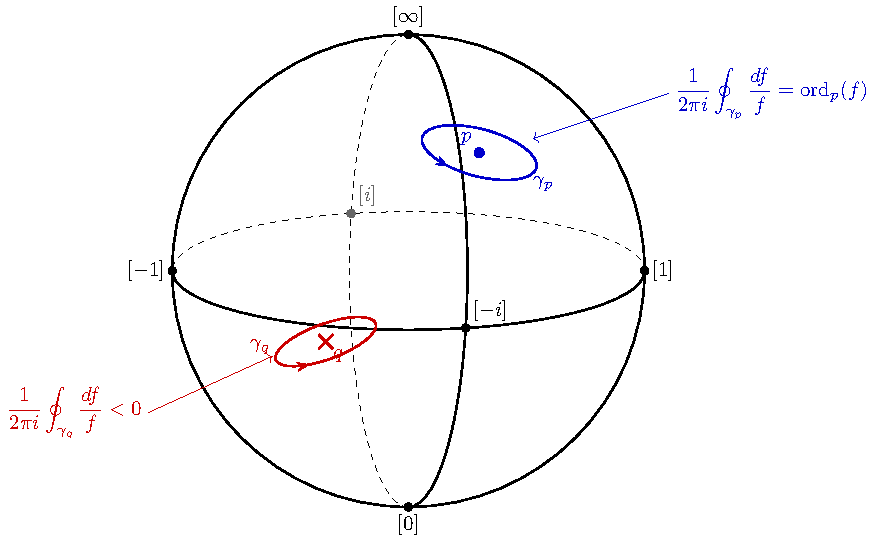
\includegraphics[scale=.9]{Riemann-Roch-Tikz/Riemann-Roch-Tikz-Divisor-1.pdf}	
\end{center}
\end{remark}

\medskip

\begin{example}
	In the coordinate $z$ on $U_0$, the function $z-a$ has a simple zero at $a\in \C$. To understand what happens at $\infty$, write $z=1/w$. Then
	\[
	z-a=\frac{1-aw}{w}.
	\]
	Near $w=0$, the factor $1-aw$ is a unit, while $1/w$ has a simple pole. Therefore
	\[
	(z-a)=[a]-[\infty].
	\]
\end{example}

\begin{example}[The divisor of $z-a$ on $\CP^1$]
Now fix $a\in \C$. On the chart $U_0$, the meromorphic function $z-a$ has a simple
zero at the point $[1:a]$, since $z=a$ there.

To determine its behavior at $\infty$, pass to the chart $U_\infty$. Since
\[
z=\frac{1}{w},
\]
we get
\[
z-a=\frac{1}{w}-a=\frac{1-aw}{w}.
\]
Near $w=0$, the factor $1-aw$ is holomorphic and nonvanishing, hence a unit.
Therefore the order of $z-a$ at $\infty$ is the same as the order of $1/w$, namely
\[
\ord_\infty(z-a)=-1.
\]
Thus $z-a$ has a simple zero at $[1:a]$ and a simple pole at $\infty$. Hence
\[
\operatorname{div}(z-a)=[a]-[\infty].
\]
\end{example}

\begin{example}
	More generally,
	\[
	\left(\frac{z-a}{z-b}\right)=[a]-[b].
	\]
\end{example}

\newpage
\lembox{\begin{lemma}
Let $X$ be a compact Riemann surface, and let $f\in \mathcal{M}(X)^\times$ be a nonzero
meromorphic function. Then \[
\sum_{p\in X}\operatorname{ord}_p(f)=0.
\]
%Equivalently, the principal divisor of $f$ has degree zero:
%\[
%\deg \operatorname{div}(f)=0.
%\]
\end{lemma}}

\begin{proof}
	Let $p_1,\dots,p_N$ are the finitely many zeros and poles of $f$.
	
	Choose pairwise disjoint coordinate disks $U_j$ around $p_j$, with local coordinate
	$z_j:U_j\to \Delta$ satisfying $z_j(p_j)=0$. For sufficiently small $r>0$, let
	\[
	D_j(r):=\{q\in U_j:|z_j(q)|<r\},
	\qquad
	C_j(r):=\partial D_j(r).
	\]
	Set
	\[
	X_r:=X\setminus \bigcup_{j=1}^N D_j(r).
	\]
	Then $X_r$ is a compact oriented surface with boundary
	\[
	\partial X_r=-\sum_{j=1}^N C_j(r),
	\]
	because each $C_j(r)$ appears with the boundary orientation induced from the
	complement of the deleted disk.
	
	On $X_r$, the function $f$ has no zeros and no poles, so the $1$-form
	\[
	\omega:=\frac{df}{f}
	\]
	is smooth on $X_r$. Since locally $\omega=d(\log f)$ on $X_r$, we have
	\[
	d\omega=0.
	\]
	Therefore, by the generalized Stokes theorem,
	\[
	0=\int_{X_r} d\omega=\int_{\partial X_r}\omega
	=-\sum_{j=1}^N \int_{C_j(r)} \frac{df}{f}.
	\]
	Hence
	\[
	\sum_{j=1}^N \int_{C_j(r)} \frac{df}{f}=0.
	\]
	
	Now compute each boundary integral locally. Since $m_j=\operatorname{ord}_{p_j}(f)$,
	in the coordinate $z_j$ we may write
	\[
	f=z_j^{m_j}u_j,
	\]
	where $u_j$ is holomorphic and nowhere vanishing on $U_j$. Thus
	\[
	\frac{df}{f}
	=
	m_j \frac{dz_j}{z_j}
	+
	\frac{du_j}{u_j}.
	\]
	Integrating around $C_j(r)$ gives
	\[
	\int_{C_j(r)} \frac{df}{f}
	=
	m_j \int_{C_j(r)} \frac{dz_j}{z_j}
	+
	\int_{C_j(r)} \frac{du_j}{u_j}.
	\]
	Because $u_j$ is nowhere vanishing on $U_j$, there exists a holomorphic branch of
	$\log u_j$ on $U_j$, so
	\[
	\frac{du_j}{u_j}=d(\log u_j),
	\]
	and therefore
	\[
	\int_{C_j(r)} \frac{du_j}{u_j}=0.
	\]
	Also,
	\[
	\int_{C_j(r)} \frac{dz_j}{z_j}=2\pi i.
	\]
	So
	\[
	\int_{C_j(r)} \frac{df}{f}=2\pi i\, m_j.
	\]
	
	Substituting into the global identity, we obtain
	\[
	0=\sum_{j=1}^N \int_{C_j(r)} \frac{df}{f}
	=2\pi i \sum_{j=1}^N m_j.
	\]
	Hence
	\[
	\sum_{j=1}^N m_j=0,
	\]
	that is,
	\[
	\sum_{p\in X}\operatorname{ord}_p(f)=0.
	\]
	This proves that every principal divisor on a compact Riemann surface has degree zero.
\end{proof}



\probox{\begin{proposition}
Every principal divisor on $\CPone$ has degree $0$.
\end{proposition}}
\begin{proof}
	Let $f=P/Q$ with coprime polynomials. If $\deg P=m$ and $\deg Q=n$, then the finite zeros contribute $m$, the finite poles contribute $-n$, and near infinity we have
	\[
	f(1/w)=\frac{P(1/w)}{Q(1/w)}\sim c\,w^{n-m},
	\]
	so
	\[
	\ord_{\infty}(f)=n-m.
	\]
	Hence
	\[
	\degd (f)=m-n+(n-m)=0.
	\]
\end{proof}

\newpage
\section{Every Divisor on $\CPone$ is Equivalent to $n[\infty]$}
\defbox[Linearly Equivalence]{\begin{definition}
	Two divisors $D,E$ are linearly equivalent, written $D\sim E$, if \[
	D-E=(f)
	\] for some nonzero meromorphic function $f$.
\end{definition}}

The key fact on $\CPone$ is that degree is the only invariant of divisor class.

\thmbox{\begin{theorem}
	Every divisor $D$ on $\CPone$ is linearly equivalent to $(\degd D)[\infty]$.
	In particular, \[
	\Pic(\CPone)\cong \mathbb Z,\qquad
	D\longmapsto \degd D.
	\]
\end{theorem}}
\begin{proof}
	Write
	\[
	D=\sum_{i=1}^r m_i[a_i]-\sum_{j=1}^s n_j[b_j]+c[\infty],
	\]
	where $a_i,b_j\in \C$ and $m_i,n_j>0$. Define
	\[
	h(z)=\frac{\prod_{i=1}^r (z-a_i)^{m_i}}{\prod_{j=1}^s (z-b_j)^{n_j}}.
	\]
	Then
	\[
	(h)=\sum_{i=1}^r m_i[a_i]-\sum_{j=1}^s n_j[b_j]-\left(\sum_{i=1}^r m_i-\sum_{j=1}^s n_j\right)[\infty].
	\]
	Therefore
	\[
	D-(h)=\left(c+\sum_{i=1}^r m_i-\sum_{j=1}^s n_j\right)[\infty]= (\degd D)[\infty].
	\]
	So $D\sim (\degd D)[\infty]$.
\end{proof}

This theorem is the concrete genus-zero form of the statement that every line bundle on $\CPone$ is some $\OO(n)$.

\newpage
\section{The Space of Meromorphic Functions $L(D)$}
Once divisors encode the zeros and poles of meromorphic functions, a natural question is
\begin{quote}
	\hl{Which meromorphic functions have zeros and poles compatible with a given divisor?}
\end{quote}
This leads to the definition \[
L(D)=\{\,f\in \mathcal{M}(X)\mid \operatorname{div}(f)+D\ge 0\,\}\cup\{0\},
\]
the space of meromorphic functions whose poles are bounded by $D$.

%\vfill
\medskip

\begin{observation}
Let $p\in X$, and let $z$ be a local coordinate with $z(p)=0$. Any nonzero meromorphic function $f$ near $p$ can be written as \[
f=z^{-m}u,\quad u(p)\neq 0,
\] for some $m\in\Z$. 
%Here, \begin{enumerate}[(i)]
%	\item $m>0$: pole of order $m$,
%	\item $m<0$: zero of order $-m$,
%	\item $m=0$: neither zero nor pole.
%\end{enumerate}
{\color{blue} Now suppose we want to allow at most a pole of order $n$ at $p$.}
Then \[
\text{$f$ has pole of order at most $n$ at $p$}\iff\text{$z^nf$ is holomorphic at $p$}.
\] 
\begin{center}
	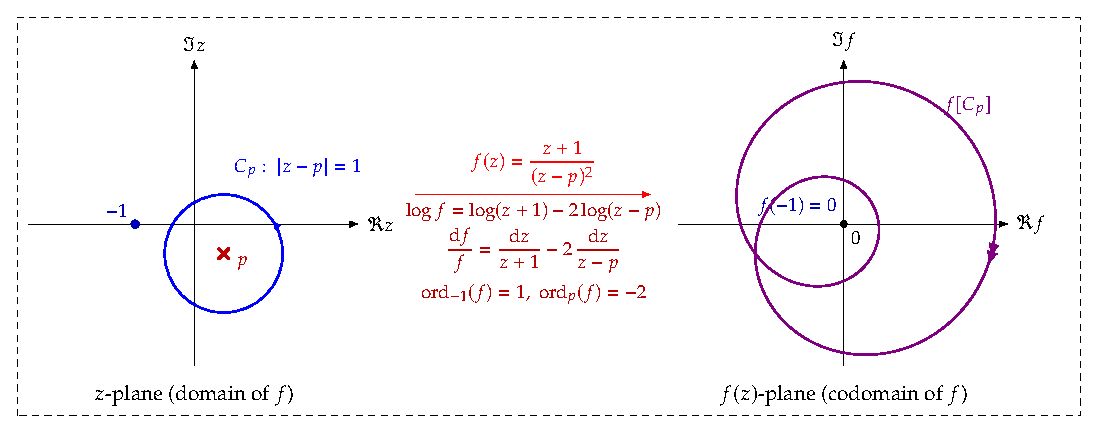
\includegraphics[width=\textwidth]{Riemann-Roch-Tikz/RIemann-Roch-Tikz-L(D)-1.pdf}
\end{center}
\begin{center}
	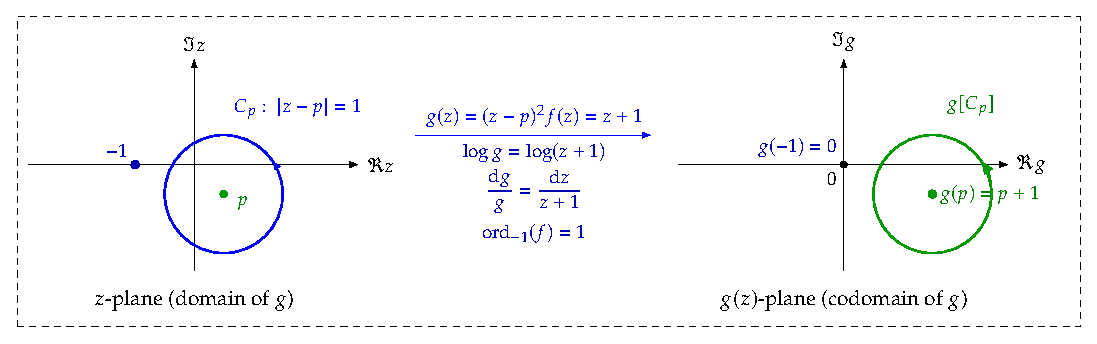
\includegraphics[width=\textwidth]{Riemann-Roch-Tikz/RIemann-Roch-Tikz-L(D)-1-2.pdf}
\end{center}
Thus \begin{align*}
\ord_p(z^nf)=\frac{1}{2\pi i}\oint_{\gamma_p}\frac{\d (z^nf)}{z^nf}
&=\frac{1}{2\pi i}\oint_{\gamma_p}\left(\frac{f\cdot nz^{n-1} \d z + z^n\cdot f'\d z }{z^nf}\right) \\
&=\frac{1}{2\pi i}\oint_{\gamma_p}\left(n\cdot \frac{\d z}{z}+\frac{\d f}{f}\right) \\
&=\frac{n}{2\pi i}\oint_{\gamma_p}\frac{\d z}{z}+\frac{1}{2\pi i}\oint_{\gamma_p}\frac{\d f}{f}\\
&=n\cdot\frac{2\pi i}{2\pi i}+\ord_p(f) \\
&=n+\ord_p(f)\geq 0,
\end{align*} so \[
\text{$f$ has pole order at most $n$ at $p$}\iff\text{$z^nf$ is holomorphic at $p$}\iff\text{$\ord_p(f)+n\geq 0$}.
\]
\end{observation}

\vfill

\defbox[Divisor Group]{\begin{definition}
Let \(X\) be a compact Riemann surface. 
The \textbf{divisor group} is %a free abelian group
\[
\operatorname{Div}(X):=
\left\{
\sum_{p\in X} n_p[p]
\;\middle|\;
n_p\in \mathbb Z,\ \text{and } n_p=0 \text{ for all but finitely many } p
\right\}.
\]
%Thus a divisor is simply a finite formal integer linear combination of points of $X$.
The group operation is addition: \[
\left(\sum_p n_p[p]\right)+\left(\sum_p m_p[p]\right)
=
\sum_p (n_p+m_p)[p].
\]
Since addition of integers is commutative, $\operatorname{Div}(X)$ is an abelian group.
\end{definition}}
%\begin{remark}
%The identity element is the zero divisor \[
%0=\sum_p 0[p],
%\] and the inverse of $
%D=\sum_p n_p[p]$ is \[
%-D=\sum_p (-n_p)[p].
%\]
%\end{remark}
\begin{remark}
Consider the following isomorphism\[
\fullfunction{\Phi}{\Div(X)}{\bigoplus_{p\in X}\Z}{\sum_{p\in X} n_p[p]}{(n_p)_{p\in X}}.
\] That is, $\operatorname{Div}(X)\cong \bigoplus_{p\in X}\mathbb Z$,
so $\operatorname{Div}(X)$ is the free abelian group generated by the points of $X$.
\end{remark}

\medskip

\begin{remark}
A divisor \(D=\sum_p n_p[p]\) is called \textbf{effective} if \(n_p\ge 0\) for all \(p\in X\), and we write \(D\ge 0\).
\end{remark}

\newpage

\defbox[Space of Meromorphic Functions (Riemann--Roch Space)]{\begin{definition}
Let \[
D=\sum_{p\in\CPone}n_p[p]\in\Div(\CP^1)
\] be a divisor on \(\CP^1\). The \textbf{space of meromorphic functions associated to \(D\)} is
\[
L(D):=\{\,f\in \mathcal M(\CP^1)^\times \mid \div(f)+D\ge 0\,\}\cup\{0\}.
\]
Equivalently,
\[
L(D)=\{\,f\in \mathcal M(\CP^1)^\times\mid \ord_p(f)\ge -n_p
\text{ for every }p\in \CP^1\,\}\cup\{0\}.
\] Its dimension is denoted by \[
\ell(D):=\dim_{\C}L(D).
\]
\end{definition}}
\begin{remark}
For a general divisor $D=\sum_{p\in X}n_p[p]$ on a compact Riemann surface $X$, \[
f\in L(D)\iff \ord_p(f)+n_p\geq0\;\text{for all $p\in X$}.
\] 	Therefore
\begin{itemize}
	\item if $n_p>0$, then $f$ may have a pole at $p$, but of order at most $n_p$;
	\item if $n_p=0$, then $f$ cannot have a pole at $p$;
	\item if $n_p<0$, then $f$ must have a zero at $p$ of order at least $-n_p$.
\end{itemize}
\end{remark}

\medskip

\medskip

\begin{remark}
%	The Riemann-Roch space $L(D)$ is the set of meromorphic functions whose poles are bounded by 
%	$D$, and adding such functions or multiplying by constants does not create worse poles than allowed.
%	The space $L(D)$ is a vector space over $\mathbb C$ because it is closed under addition and scalar multiplication, hence it is a $\mathbb C$-subspace of the field of meromorphic functions $\mathcal M(\mathbb{CP}^1)\simeq\C(z)$.
	Take $D=\sum_{p\in X} n_p[p]$ and consider $L(D)$.
%	\begin{align*}
%	L(D)&=\{\,f\in \mathcal M(X)^\times \mid \operatorname{div}(f)+D\ge 0\,\}\cup\{0\}\\
%	&=\{\,f\in \mathcal M(X)^\times \mid \textstyle\sum_{p\in X}\bigl(\ord_p(f)+n_p\bigr)[p]\ge 0\,\}\cup\{0\} \\
%	&=\{\,f\in \mathcal M(X)^\times \mid \ord_p(f)+n_p[p]\ge 0\,\text{ for all $p\in X$}\}\cup\{0\}.
%	\end{align*} 
	Then \begin{enumerate}[(i)]
		\item By definition, $0\in L(D)$.
		\item Let $f\in L(D)$ and $c\in\mathbb C$. If $c=0$, then $cf=0\in L(D)$. If $c\neq 0$, then
		\[
		\ord_p(cf)
		=
		\frac{1}{2\pi i}\oint_{\gamma_p}\frac{\d(cf)}{cf}
		=
		\frac{1}{2\pi i}\oint_{\gamma_p}\frac{\d f}{f}
		=
		\ord_p(f).
		\] for every point $p\in X$. Then \[
		\ord_p(f)+n_p\ge 0\implies\ord_p(cf)+n_p\ge 0
		\] for all $p\in X$, hence $cf\in L(D)$.
		\item Let $f,g\in L(D)$ with $f+g\neq 0$. Fix a point $p\in X$. Define
		\[
		m:=\min\{\ord_p(f),\ord_p(g)\}.
		\]
		Choose a local coordinate $z$ centered at $p$. Then \[
		f=z^m u,
		\qquad
		g=z^m v,
		\]
		where $u$ and $v$ are holomorphic near $p$, and at least one of $u(p),v(p)$ is nonzero. Then
		\[
		\ord_p(f+g)=\ord_p(z^m(u+v))=m+\ord_p(u+v).
		\] Since $u+v$ is holomorphic ($\ord_p(u+v)\geq 0$), we have
		\[
		\ord_p(f+g)\ge m=\min\{\ord_p(f),\ord_p(g)\}.
		\]
		Since $f,g\in L(D)$, we have
		\[
		\ord_p(f)+n_p\ge 0
		\quad\text{and}\quad
		\ord_p(g)+n_p\ge 0,
		\] so
		\[
		m+n_p=\min\{\ord_p(f),\ord_p(g)\}+n_p\ge 0.
		\]
		Therefore
		\[
		\ord_p(f+g)+n_p\ge m+n_p\ge 0,
		\]
		so $f+g\in L(D)$.
	\end{enumerate}
	Hence $L(D)$ is a vector space over $\mathbb C$. If $X$ is compact, this vector space is in fact finite-dimensional, and we write \[
	\ell(D):=\dim_{\mathbb C}L(D).
	\]
\end{remark}

\medskip
%\begin{example}
%Let $D=n[\infty]\in \Div(\CP^1)$ for some $n\in\Z$. Consider \[
%L(n[\infty])=\{\,f\in \mathcal M(\CP^1)^\times \mid \div(f)+n[\infty]\ge 0\,\}\cup\{0\}.
%\] 
%%the space of meromorphic functions on $\mathbb{CP}^1$ that are allowed to have a pole only at $\infty$, and there of order at most $n$.
%Then \begin{align*}
%f\in L(n[\infty])&\implies \sum_{p\in\CPone}\ord_p(f)[p] + n[\infty]\geq 0\\
%&\implies \left(\sum_{p\in\C}\ord_p(f)[p]\right)+(\ord_\infty(f)+n)[\infty]\geq 0\\
%&\implies \begin{cases}
%	\ord_{p\neq\infty}(f)\geq 0 \\
%	\ord_\infty(f)+n\geq 0
%\end{cases}.
%\end{align*}
%Thus, \begin{align*}
%L(n[\infty])&=\{\,f\in \mathcal M(\CP^1)^\times \mid \div(f)+n[\infty]\ge 0\,\}\cup\{0\}\\
%&=\{\,f\in \mathcal M(\CP^1)\mid \ord_p(f)\ge 0
%\text{ for all }p\neq \infty,\ \ord_\infty(f)\ge -n\,\}.
%%&=\{\text{meromorphic functions on $\CPone$ with no poles except at $\infty$, and there of order $\leq n$}\}
%\end{align*} 
%%Hence, $L(n[\infty])$ is the space of meromorphic functions on $\mathbb{CP}^1$ with no poles except at $\infty$, and there of order at most $n$.
%\end{example}

\medskip

\begin{example}[Computing $L(D)$ and $\ell(D)$]
\; \begin{enumerate}[(1)]
	\item {\color{blue} Let $D=0$ (zero divisor).} Then \[
	L(0)=\{\,f\in\mathcal M(\mathbb{CP}^1)^\times\mid \operatorname{div}(f)\ge 0\,\}\cup\{0\}=\{\,f\in\mathcal M(\mathbb{CP}^1)^\times\mid \ord_p(f)\ge 0\,\text{ for all $p\in \CP^1$}\}\cup\{0\}.
	\] So $f$ has no poles anywhere on $\mathbb{CP}^1$. Hence $f$ is holomorphic everywhere on the compact Riemann surface $\mathbb{CP}^1$, so $f$ must be constant. Therefore
	\[
	L(0)=\mathbb C\quad\text{and}\quad\ell(0)=\dim_\C L(0)=1.
	\]
	\item {\color{blue} Let $D=[0]$ (simple zero at $0$).} Then \begin{align*}
	L([0])&=\{\,f\in\mathcal M(\mathbb{CP}^1)^\times\mid \operatorname{div}(f)+[0]\ge 0\,\}\cup\{0\}\\
	&=\{\,f\in\mathcal M(\mathbb{CP}^1)^\times\mid \textstyle\sum_{p\in\C\setminus\{0\}}\ord_p[p]+(\ord_0(f)+1)[0]+(\ord_\infty(f))[\infty]\ge 0\,\}\cup\{0\}\\
	&=\{\,f\in\mathcal M(\mathbb{CP}^1)^\times\mid \ord_{p\notin\{0,\infty\}}(f)\geq 0; \,\ord_{0}(f)\geq -1; \,\ord_{\infty}(f)\geq 0\}\cup\{0\} \\
	&=\set{\,f\in\mathcal M(\mathbb{CP}^1)^\times\mid \substack{\text{\normalsize\color{red} $f$ has no pole at $\infty$}\\ \text{\normalsize\color{orange} $f$ may have pole of order $\leq 1$ at $0$}}}\cup\{0\}
	\end{align*}
	Let \[
	\color{orange}f(z)=\frac{P(z)}{z},\quad P(z)\in\C[z].
	\] Note that \begin{align*}
		P(z)&=a_0+a_1z+\cdots+a_{\deg P}z^{\deg P}\quad(a_{\deg P}\neq 0),\\
		P(1/w)&=a_0+a_1w^{-1}+\cdots+a_{\deg P}w^{-\deg P}.
	\end{align*}
	Since no pole is allowed at $\infty$, we require
	\[
	\color{red}\ord_\infty(f)=\ord_{w=0}(wP(1/w))=1-\deg P\ge 0,
	\]
	so $\deg P\le 1$. Thus $P(z)=az+b$ ($a,b\in\C$)
	and therefore \[
	f(z)=\frac{az+b}{z}=a+\frac{b}{z}.
	\]
	Hence
	\[
	L([0])=\set{a+\frac{b}{z}:a,b\in\C}=\operatorname{span}_\C\left\{1,\frac1z\right\}
	\quad\text{so}\quad
	\ell([0])=2.
	\]
	\item {\color{blue} Let $D=[0]+[1]$.} Then
	\begin{align*}
		&L([0]+[1])\\
		&=\{\,f\in\mathcal M(\mathbb{CP}^1)^\times\mid \operatorname{div}(f)+[0]+[1]\ge 0\,\}\cup\{0\}\\
		&=\{\,f\in\mathcal M(\mathbb{CP}^1)^\times\mid \textstyle\sum_{p\in\C\setminus\{0,1\}}\ord_p[p]+(\ord_0(f)+1)[0]+(\ord_1(f)+1)[1]+(\ord_\infty(f))[\infty]\ge 0\,\}\cup\{0\}\\
		&=\{\,f\in\mathcal M(\mathbb{CP}^1)^\times\mid \ord_{p\notin\{0,\infty\}}(f)\geq 0; \,\ord_{0}(f)\geq -1;\,\ord_{1}(f)\geq -1; \,\ord_{\infty}(f)\geq 0\}\cup\{0\} \\
		&=\set{\,f\in\mathcal M(\mathbb{CP}^1)^\times\mid \substack{\text{\normalsize\color{red} $f$ has no pole at $\infty$}\\ \text{\normalsize\color{orange} $f$ may have pole of order $\leq 1$ at $0$}\\ \text{\normalsize\color{orange} $f$ may have pole of order $\leq 1$ at $1$}}}\cup\{0\}
	\end{align*}
	Let \[
	\color{orange}f(z)=\frac{P(z)}{z(z-1)},\quad P(z)\in\C[z].
	\]
	Since no pole is allowed at $\infty$, we require
	\[
	\color{red}\ord_\infty(f)=\ord_{w=0}\left(w\cdot\frac{w}{1-w}\cdot P(1/w)\right)=\ord_{w=0}\left(w^2\cdot\frac{1}{1-w}\cdot P(1/w)\right)=2-\deg P\ge 0,
	\]
	so $\deg P\le 2$. Thus $P(z)=az^2+bz+c$ ($a,b,c\in\C$)
	and therefore \[
	f(z)=\frac{az^2+bz+c}{z(z-1)}=A+\frac{B}{z}+\frac{C}{z-1}.
	\] Since \[
	az^2+bz+c=Az(z-1)+B(z-1)+Cz=Az^2+(-A+B+C)z-B,
	\] we have \[
	\begin{cases}
		A=a\\
		-A+B+C=b\\
		-B=c
	\end{cases}\implies
	\begin{cases}
	A=a\\
	B=-c\\
	C=a+b+c
	\end{cases}.
	\] Thus 
	\[
	f(z)=a-\frac{c}{z}+\frac{a+b+c}{z-1},
	\qquad a,b,c\in\mathbb C.
	\]
	Therefore
	\[
	L([0]+[1])=\set{a-\frac{c}{z}+\frac{a+b+c}{z-1}:a,b,c\in\C}=\operatorname{span}\left\{1,\frac1z,\frac1{z-1}\right\}\quad\text{and}\quad\ell([0]+[1])=3.
	\]	
	\item {\color{blue} Let $D=[\infty]$.} 
	Then
	\begin{align*}
		L([\infty])&=\{\,f\in\mathcal M(\mathbb{CP}^1)^\times\mid \operatorname{div}(f)+[\infty]\ge 0\,\}\cup\{0\}\\
		&=\{\,f\in\mathcal M(\mathbb{CP}^1)^\times\mid \textstyle\sum_{p\in\C}\ord_p[p]+(\ord_\infty(f)+1)[\infty]\ge 0\,\}\cup\{0\}\\
		&=\{\,f\in\mathcal M(\mathbb{CP}^1)^\times\mid \ord_{p\in\C}(f)\geq 0; \,\ord_{\infty}(f)\geq -1\}\cup\{0\} \\
		&=\set{\,f\in\mathcal M(\mathbb{CP}^1)^\times\mid \substack{\text{\normalsize\color{red} $f$ may have a pole of order $\leq 1$ at $\infty$}\\ \text{\normalsize\color{orange} $f$ has no pole at any finite point $p\in\C$}}}\cup\{0\}
	\end{align*}
	Let \[
	\color{orange} f(z)=P(z)\quad\text{with}\quad P(z)\in\C[z].
	\]
	Since $f$ may have a pole of order at most 1 at $\infty$, we require \[
	\color{red}\ord_{\infty}(f)=\ord_{w=0}\left(P(1/w)\right)=-\deg P\ge -1,
	\] so $\deg P\leq 1$. Thus $P(z)=az+b$ ($a,b\in\C$)
	and therefore \[
	f(z)=az+b,\quad a,b\in\C.
	\] Hence
	\[
	L([\infty])=\set{az+b:a,b\in\C}=\operatorname{span}_\C\{1,z\}
	\quad\text{and}\quad
	\ell([\infty])=2.
	\]
	\item {\color{blue} Let $D=2[\infty]$.} Then
	\[
	L(2[\infty])
	=
	\{\,f\in\mathcal M(\mathbb{CP}^1)\mid \operatorname{div}(f)+2[\infty]\ge 0\,\}\cup\{0\}.
	\]
	Thus $f$ has no poles on $\mathbb C$ and at most a double pole at $\infty$.
	Equivalently, $f$ is a polynomial of degree at most $2$. Therefore
	\[
	L(2[\infty])=\set{az^2+bz+c:a,b,c\in\C}=\operatorname{span}_\C\{1,z,z^2\}
	\quad\text{and}\quad
	\ell(2[\infty])=3.
	\]
	\newpage
	\item {\color{blue} Let $D=[0]+[\infty]$.} Then
	\begin{align*}
		L([0]+[\infty])&=\{\,f\in\mathcal M(\mathbb{CP}^1)^\times\mid \operatorname{div}(f)+[0]+[\infty]\ge 0\,\}\cup\{0\}\\
		&=\{\,f\in\mathcal M(\mathbb{CP}^1)^\times\mid \textstyle\sum_{p\in\C\setminus\{0\}}\ord_p[p]+(\ord_0(f)+1)[0]+(\ord_\infty(f)+1)[\infty]\ge 0\,\}\cup\{0\}\\
		&=\{\,f\in\mathcal M(\mathbb{CP}^1)^\times\mid \ord_{p\in\C\setminus\{0\}}(f)\geq 0;\,\ord_0(f)\geq -1; \,\ord_{\infty}(f)\geq -1\}\cup\{0\} \\
		&=\set{\,f\in\mathcal M(\mathbb{CP}^1)^\times\mid \substack{\text{\normalsize\color{red} $f$ may have a pole of order $\leq 1$ at $\infty$}\\ \text{\normalsize\color{orange} $f$ may have a pole of order $\leq 1$ at $0$}}}\cup\{0\}
	\end{align*}
	Let \[
	\color{orange} f(z)=\frac{P(z)}{z}\quad\text{with}\quad P(z)\in\C[z].
	\]
	Since $f$ may have a pole of order at most 1 at $\infty$, we require \[
	\color{red}\ord_{\infty}(f)=\ord_{w=0}\left(wP(1/w)\right)=1-\deg P\ge -1,
	\] so $\deg P\leq 2$. Thus $P(z)=az^2+bz+c$ ($a,b,c\in\C$)
	and therefore \[
	f(z)=\frac{az^2+bz+c}{z}=az+b+\frac{c}{z},\quad a,b,c\in\C.
	\] Hence
	\[
	L([0]+[\infty])=\set{az+b+c/z:a,b,c\in\C}=\operatorname{span}\left\{1,z,\frac1z\right\}
	\quad\text{and}\quad
	\ell([0]+[\infty])=3.
	\]
	\item[]
	\item[]
	\item[]
	\item {\color{blue} Let $D=[\infty]-[1]$.} Then
	\begin{align*}
		L([\infty]-[1])&=\{\,f\in\mathcal M(\mathbb{CP}^1)^\times\mid \operatorname{div}(f)+[\infty]-[1]\ge 0\,\}\cup\{0\}\\
		&=\{\,f\in\mathcal M(\mathbb{CP}^1)^\times\mid \textstyle\sum_{p\in\C\setminus\{0\}}\ord_p[p]+(\ord_0(f)-1)[0]+(\ord_\infty(f)+1)[\infty]\ge 0\,\}\cup\{0\}\\
		&=\{\,f\in\mathcal M(\mathbb{CP}^1)^\times\mid \ord_{p\in\C\setminus\{0\}}(f)\geq 0;\,\ord_0(f)\geq 1; \,\ord_{\infty}(f)\geq -1\}\cup\{0\} \\
		&=\set{\,f\in\mathcal M(\mathbb{CP}^1)^\times\mid \substack{\text{\normalsize\color{red} $f$ may have a pole of order at most $1$ at $\infty$}\\ \text{\normalsize\color{orange} $f$ has a zero of order at least $1$ at $1$}}}\cup\{0\}
	\end{align*}
	Let \[
	\color{orange} f(z)=(z-1)P(z)\quad\text{with}\quad P(z)\in\C[z].
	\]
	Since $f$ may have a pole of order at most 1 at $\infty$, we require \[
	\color{red}\ord_{\infty}(f)=\ord_{w=0}\left(\frac{1-w}{w}\cdot P(1/w)\right)=-1-\deg P\ge -1,
	\] so $\deg P\leq 0$. Thus $P(z)=a$ ($a\in\C$)
	and therefore \[
	f(z)=a(z-1),\quad a\in\C.
	\] Hence \[
	L([\infty]-[1])=\set{a(z-1):a\in\C}=\operatorname{span}_\C\left\{z-1\right\}
	\quad\text{and}\quad
	\ell([\infty]-[1])=1.
	\]
	\item {\color{blue} Let $D=2[\infty]-[1]$.} Then
	\begin{align*}
		L(2[\infty]-[1])&=\set{\,f\in\mathcal M(\mathbb{CP}^1)^\times\mid \substack{\text{\normalsize\color{red} $f$ may have a pole of order at most $2$ at $\infty$}\\ \text{\normalsize\color{orange} $f$ has a zero of order at least $1$ at $1$}}}\cup\{0\}
	\end{align*}
	Let \[
	\color{orange} f(z)=(z-1)P(z)\quad\text{with}\quad P(z)\in\C[z].
	\]
	Since $f$ may have a pole of order at most 2 at $\infty$, we require \[
	\color{red}\ord_{\infty}(f)=\ord_{w=0}\left(\frac{1-w}{w}\cdot P(1/w)\right)=-1-\deg P\ge -2,
	\] so $\deg P\leq 1$. Thus $P(z)=az+b$ ($a,b\in\C$)
	and therefore \[
	f(z)=(z-1)(az+b)=az^2+(-a+b)z+b,\quad a,b\in\C.
	\] Then \[
	L(2[\infty]-[1])\subseteq\operatorname{span}_\C\{1,z,z^2\}\quad\text{but}\quad L(2[\infty]-1)\neq\operatorname{span}_\C\{1,z,z^2\}.
	\] since $L(2[\infty]-[1])$ has the condition that the function must must be vanish at $z=1$. Thus, \[
	f(z)=(z-1)(az+b)=az(z-1)+b(z-1),\quad a,b\in\C.
	\]
	Hence \[
	L(2[\infty]-[1])=\set{az(z-1)+b(z-1):a,b\in\C}=\operatorname{span}_\C\left\{z-1,z(z-1)\right\}
	\quad\text{and}\quad
	\ell(2[\infty]-[1])=2.
	\] 
	\newpage
	\item {\color{blue} Let $D=2[\infty]-[0]-[1]$.} Then
	\begin{align*}
		&L(2[\infty]-[0]-[1])\\
		&=\{\,f\in\mathcal M(\mathbb{CP}^1)^\times\mid \operatorname{div}(f)+2[\infty]-[0]-[1]\ge 0\,\}\cup\{0\}\\
		&=\{\,f\in\mathcal M(\mathbb{CP}^1)^\times\mid \textstyle\sum_{p\in\C\setminus\{0,1\}}\ord_p[p]+(\ord_0(f)-1)[0]+(\ord_1(f)-1)[1]+(\ord_\infty(f)+2)[\infty]\ge 0\,\}\cup\{0\}\\
		&=\{\,f\in\mathcal M(\mathbb{CP}^1)^\times\mid \ord_{p\in\C\setminus\{0,1\}}(f)\geq 0;\,\ord_0(f)\geq 1;\,\ord_1(f)\geq 1; \,\ord_{\infty}(f)\geq -2\}\cup\{0\} \\
		&=\set{\,f\in\mathcal M(\mathbb{CP}^1)^\times\mid \substack{\text{\normalsize\color{red} $f$ may have a pole of order at most $2$ at $\infty$}\\ \text{\normalsize\color{orange} $f$ has a zero of order at least $1$ at $0$}\\ \text{\normalsize\color{orange} $f$ has a zero of order at least $1$ at $1$}}}\cup\{0\}
	\end{align*}
	Let \[
	\color{orange} f(z)=z(z-1)P(z)\quad\text{with}\quad P(z)\in\C[z].
	\]
	Since $f$ may have a pole of order at most 2 at $\infty$, we require \[
	\color{red}\ord_{\infty}(f)=\ord_{w=0}\left(\frac{1}{w}\cdot\frac{1-w}{w}\cdot P(1/w)\right)=-2-\deg P\ge -2,
	\] so $\deg P\leq 0$. Thus $P(z)=a$ ($a\in\C$)
	and therefore $f(z)=az(z-1)$ ($a\in\C$). Hence \[
	L(2[\infty]-[0]-[1])
	=\{az(z-1):a\in\C\}=
	\operatorname{span}_\C\{z(z-1)\}
	\quad\text{and}\quad
	\ell(2[\infty]-[0]-[1])=1.
	\]
	
	\item {\color{blue} Let $D=[0]-[\infty]$.} Then
	\begin{align*}
		L([0]-[\infty])&=\{\,f\in\mathcal M(\mathbb{CP}^1)^\times\mid \operatorname{div}(f)+[0]-[\infty]\ge 0\,\}\cup\{0\}\\
		&=\{\,f\in\mathcal M(\mathbb{CP}^1)^\times\mid \textstyle\sum_{p\in\C\setminus\{0\}}\ord_p[p]+(\ord_0(f)+1)[0]+(\ord_\infty(f)-1)[\infty]\ge 0\,\}\cup\{0\}\\
		&=\{\,f\in\mathcal M(\mathbb{CP}^1)^\times\mid \ord_{p\in\C\setminus\{0\}}(f)\geq 0;\,\ord_0(f)\geq -1; \,\ord_{\infty}(f)\geq 1\}\cup\{0\} \\
		&=\set{\,f\in\mathcal M(\mathbb{CP}^1)^\times\mid \substack{\text{\normalsize\color{red} $f$ has a zero of order at least $1$ at $\infty$}\\ \text{\normalsize\color{orange} $f$ may have a pole of order at most $1$ at $0$}}}\cup\{0\}
	\end{align*}
	Let \[
	\color{orange} f(z)=\frac{P(z)}{z}\quad\text{with}\quad P(z)\in\C[z].
	\]
	Since $f$ has a zero of order at least 1 at $\infty$, we require \[
	\color{red}\ord_{\infty}(f)=\ord_{w=0}\left(w\cdot P(1/w)\right)=1-\deg P\ge 1,
	\] so $\deg P\leq 0$. Thus $P(z)=a$ ($a\in\C$)
	and therefore $f(z)=a/z$ ($a\in\C$). Hence \[
	L([0]-[\infty])=\{a/z:a\in\C\}=\operatorname{span}_\C\left\{\frac{1}{z}\right\}
	\quad\text{and}\quad
	\ell([0]-[\infty])=1.
	\]
\end{enumerate}
\end{example}

\newpage
\begin{note}
	Since every divisor on $\CP^1$ is equivalent to $n[\infty]$, it suffices to compute $L(n[\infty])$.
\end{note}

\probox{
	\begin{proposition}
		Let $D=n[\infty]\in\Div(\CPone)$ for some $n\in\Z$. If $n\ge 0$, then
		\[
		L(n[\infty])=\operatorname{span}_\C\set{1,z,z^2,\dots,z^n}.
%			\{\text{polynomials in }z\text{ of degree }\le n\}.
		\] If $n<0$, then $L(n[\infty])=0$.
		In particular,
		\[
		\ellD(n[\infty])=
		\begin{cases}
			n+1,& n\ge 0, \\
			0,& n<0.
		\end{cases}
		\]
\end{proposition}}
\begin{proof}
	Take a divisor $D=n[\infty]\in\Div(\CPone)$ with $n\in\Z$.  Then
	\begin{align*}
		L(n[\infty])&=\{\,f\in\mathcal M(\mathbb{CP}^1)^\times\mid \operatorname{div}(f)+n[\infty]\ge 0\,\}\cup\{0\}\\
		&=\{\,f\in\mathcal M(\mathbb{CP}^1)^\times\mid \textstyle\sum_{p\in\C}\ord_p[p]+(\ord_\infty(f)+n)[\infty]\ge 0\,\}\cup\{0\}\\
		&=\{\,f\in\mathcal M(\mathbb{CP}^1)^\times\mid \ord_{p\in\C}(f)\geq 0; \,\ord_{\infty}(f)\geq -n\}\cup\{0\}.
	\end{align*}\begin{enumerate}[(i)]
		\item Assume that $n\geq 0$. Then
		\begin{align*}
			&\{\,f\in\mathcal M(\mathbb{CP}^1)^\times\mid \ord_{p\in\C}(f)\geq 0; \,\ord_{\infty}(f)\geq -n\}\cup\{0\} \\
			=&\set{\,f\in\mathcal M(\mathbb{CP}^1)^\times\mid \substack{\text{\normalsize\color{red} $f$ may have a pole of order at most $n$ at $\infty$}\\ \text{\normalsize\color{orange} $f$ has no pole at $p\in\C$}}}\cup\{0\}
		\end{align*}
		Let \[
		\color{orange} f(z)=P(z)\quad\text{with}\quad P(z)\in\C[z].
		\]
		Since $f$ may have a pole of order at most $n$ at $\infty$, we require \[
		\color{red}\ord_{\infty}(f)=\ord_{w=0}\left(P(1/w)\right)=-\deg P\ge -n,
		\] so $\deg P\leq n$. Thus $P(z)=a$ ($a\in\C$)
		and therefore $f(z)=a_0+a_1z+\cdots+a_nz^n$ ($a_i\in\C$). Hence \[
		L(n[\infty])=\operatorname{span}_\C\left\{1,z,z^2,\dots,z^n\right\}
		\quad\text{and}\quad
		\ell(n[\infty])=n+1.
		\]
		\item Assume that $n<0$. Then \begin{align*}
			&\{\,f\in\mathcal M(\mathbb{CP}^1)^\times\mid \ord_{p\in\C}(f)\geq 0; \,\ord_{\infty}(f)\geq -n\}\cup\{0\} \\
			=&\set{\,f\in\mathcal M(\mathbb{CP}^1)^\times\mid \substack{\text{\normalsize\color{red} $f$ has a zero of order at least $-n$ at $\infty$}\\ \text{\normalsize\color{orange} $f$ has no pole at $p\in\C$}}}\cup\{0\}
		\end{align*}
		Let \[
		\color{orange} f(z)=P(z)\quad\text{with}\quad P(z)\in\C[z].
		\]
		Since $f$ has a zero of order at least $n$ at $\infty$, we require \[
		\color{red}\ord_{\infty}(f)=\ord_{w=0}\left(P(1/w)\right)=-\deg P\ge -n,
		\] so $\deg P\leq n$. Since $P(z)\in\C[z]$, $P(z)\equiv 0$ therefore $f(z)=0$. Hence \[
		L(n[\infty])=\{0\}
		\quad\text{and}\quad
		\ell(n[\infty])=0.
		\]
	\end{enumerate}
%	If $n<0$, then $f\in L(n[\infty])$ would have to vanish at infinity to order at least $-n$, while having no poles anywhere. So $f$ would be a holomorphic function on the compact surface $\CPone$ vanishing at a point. Since global holomorphic functions on $\CPone$ are constant, we get $f=0$.
\end{proof}

\medskip
\thmbox{\begin{theorem}
	Let $X$ be a compact Riemann surface, and let $D,D'\in\Div(X)$ \[
	D\sim D'\quad\text{implies}\quad L(D)\simeq L(D').
	\] 
%	and let $D,D'\in \Div(X)$ be linearly equivalent divisors. Then there is a natural isomorphism of $\C$-vector spaces
%	\[
%	L(D)\cong L(D').
%	\]
	In particular, $\ell(D)=\ell(D').$
\end{theorem}}
\begin{proof}
	Since $D\sim D'$,\[
	\exists g\in\mathcal M(X)^\times\quad\text{such that}\quad D=D'+\div(g).
	\]
	Define \[
	\fullfunction{\Phi_g}{L(D)}{L(D')}{f}{gf}.
	\] Let $f\in L(D)$. Then $\div(f)+D\ge 0$, and so \[
	\div\!\left(gf\right)+D'
	=(\div(g)+\div(f))+(D-\div(g))
	=
	\div(f)+D\ge 0.
	\]
	Hence $gf\in L(D')$. So $\Phi_h$ is well-defined. Let $f,f'$ and $a,b\in\C$ then \[
	\Phi_g(af+bf')=g(af+bf')=agf+bgf'=a\Phi_g(f)+b\Phi_g(b),
	\] so $\Phi_g$ be $\C$-linear. Define also \[
	\fullfunction{\Psi_g}{L(D)}{L(D')}{f}{\frac{f}{g}}.
	\]
	We check that $\Psi_h$ is well-defined. If $g\in L(D')$, then
	\[
	\div(g)+D'\ge 0.
	\]
	Since $D'=D+\div(h)$, we get
	\[
	\div(gh)+D
	=
	\div(g)+\div(h)+D
	=
	\div(g)+D'\ge 0.
	\]
	Thus
	\[
	gh\in L(D),
	\]
	so $\Psi_h$ is well-defined.
	
	Finally, for $f\in L(D)$ and $g\in L(D')$,
	\[
	\Psi_h(\Phi_h(f))=\left(\frac{f}{h}\right)h=f,
	\qquad
	\Phi_h(\Psi_h(g))=\frac{gh}{h}=g.
	\]
	Therefore $\Phi_h$ and $\Psi_h$ are inverse linear maps. Hence
	\[
	L(D)\cong L(D').
	\]
	
	Taking dimensions, we conclude that
	\[
	\ell(D)=\ell(D').
	\]
\end{proof}

\corbox{\begin{corollary}
		For any divisor $D$ on $\CPone$,
		\[
		\ellD(D)=
		\begin{cases}
			\deg D+1,& \degd D\ge 0,\\
			0,& \degd D<0.
		\end{cases}
		\]
\end{corollary}}
\begin{remark}
The condition is on $\deg D$, not on whether $D$ is effective.
\end{remark}
\begin{proof}
	Note that $D\sim (\degd D)[\infty]$ on $\CP^1$.
	%	Since $D\sim (\degd D)[\infty]$, the spaces $L(D)$ and $L((\degd D)[\infty])$ are naturally isomorphic by multiplication with a meromorphic function that realizes the equivalence. Hence dimensions agree, and the previous proposition applies.
\end{proof}
The correct formula on $\mathbb{CP}^1$ is
\[
\ell(D)=
\begin{cases}
	\deg D+1,& \deg D\ge 0,\\[4pt]
	0,& \deg D<0.
\end{cases}
\]


The reason is that if $D\sim D'$, then $L(D)\cong L(D')$. Indeed, if
\[
D-D'=\operatorname{div}(h)
\]
for some nonzero meromorphic function $h$, then multiplication by $h$ defines an isomorphism
\[
L(D)\longrightarrow L(D'),\qquad f\longmapsto hf.
\]
For if $f\in L(D)$, then
\[
\operatorname{div}(f)+D\ge 0,
\]
and therefore
\[
\operatorname{div}(hf)+D'
=
\operatorname{div}(h)+\operatorname{div}(f)+D'
=
(D-D')+\operatorname{div}(f)+D'
=
\operatorname{div}(f)+D\ge 0.
\]
Hence $hf\in L(D')$, and so
\[
\ell(D)=\ell(D').
\]

Now on $\mathbb{CP}^1$, every divisor $D$ is linearly equivalent to $(\deg D)[\infty]$. Indeed, for every finite point $a\in\mathbb C$,
\[
\operatorname{div}(z-a)=[a]-[\infty],
\]
so
\[
[a]\sim [\infty].
\]
Therefore any divisor $D$ satisfies
\[
D\sim (\deg D)[\infty].
\]

It follows that
\[
\ell(D)=\ell((\deg D)[\infty]).
\]
Since
\[
\ell(n[\infty])=
\begin{cases}
	n+1,& n\ge 0,\\
	0,& n<0,
\end{cases}
\]
we conclude that
\[
\ell(D)=
\begin{cases}
	\deg D+1,& \deg D\ge 0,\\[4pt]
	0,& \deg D<0.
\end{cases}
\]

\newpage
The identity
\[
L(D)=H^0(X,\mathcal O_X(D))
\]
comes from the definition of the sheaf $\mathcal O_X(D)$. If
\[
D=\sum_p n_p[p],
\]
then for an open set $U\subseteq X$ one defines
\[
\mathcal O_X(D)(U)
=
\{\,f\in \mathcal M_X(U)\mid \operatorname{div}(f)|_U+D|_U\ge 0\,\},
\]
where $\mathcal M_X(U)$ denotes the meromorphic functions on $U$. Thus a section of $\mathcal O_X(D)$ over $U$ is precisely a meromorphic function whose poles and zeros are compatible with the divisor $D$ on $U$.

Taking global sections gives
\[
H^0(X,\mathcal O_X(D))
=
\{\,f\in \mathcal M(X)\mid \operatorname{div}(f)+D\ge 0\,\},
\]
which is exactly the Riemann--Roch space $L(D)$.

Now let $X=\mathbb{CP}^1$ and $D=n[\infty]$. Then
\[
H^0(\mathbb{CP}^1,\mathcal O(n[\infty]))
=
L(n[\infty]).
\]
A function $f$ lies in $L(n[\infty])$ if and only if it has no poles on $\mathbb C$ and has a pole of order at most $n$ at $\infty$. Therefore $f$ must be a polynomial of degree at most $n$. Hence
\[
H^0(\mathbb{CP}^1,\mathcal O(n[\infty]))
=
L(n[\infty])
=
\operatorname{span}\{1,z,z^2,\dots,z^n\}
\qquad (n\ge 0).
\]

Using the local coordinate $w=1/z$ near $\infty$, one has
\[
z^k=w^{-k},
\]
so $z^k$ has a pole of order $k$ at $\infty$. This explains why exactly the functions
\[
1,z,\dots,z^n
\]
occur as global sections of $\mathcal O(n[\infty])$.


\newpage
For now, you can think of
\[
H^0(X,\mathcal F)
\]
as meaning simply the space of \emph{global sections} of the sheaf $\mathcal F$. In other words,
\[
H^0(X,\mathcal F)=\mathcal F(X).
\]

So if $\mathcal O_X(D)$ is the sheaf whose sections over an open set $U$ are meromorphic functions on $U$ compatible with the divisor $D$, then
\[
H^0(X,\mathcal O_X(D))
\]
means the meromorphic functions on all of $X$ compatible with $D$.

Thus
\[
H^0(X,\mathcal O_X(D))
=
\{\,f\in\mathcal M(X)\mid \operatorname{div}(f)+D\ge 0\,\}
=
L(D).
\]

So the identity
\[
L(D)=H^0(X,\mathcal O_X(D))
\]
is just saying that the Riemann--Roch space $L(D)$ is the space of global sections of $\mathcal O_X(D)$.

For example, on $\mathbb{CP}^1$,
\[
H^0(\mathbb{CP}^1,\mathcal O_{\mathbb{CP}^1}(n[\infty]))
=
L(n[\infty])
=
\operatorname{span}\{1,z,z^2,\dots,z^n\}.
\]

%\begin{definition}
%	Let \(D\in \Div(\CP^1)\). The Riemann--Roch space associated to \(D\) is
%	\[
%	L(D):=H^0(\CP^1,\mathcal O(D))
%	=\{\,f\in \mathcal M(\CP^1)\mid \div(f)+D\ge 0\,\}.
%	\]
%\end{definition}


\newpage
Yes, but only as an analogy. The notation
\[
H^0(X,\mathcal O_X(D))
\]
is not de Rham cohomology; it is sheaf cohomology. However, there is a useful comparison.

In de Rham theory,
\[
H^0_{\mathrm{dR}}(X)=\ker\bigl(d:\Omega^0(X)\to \Omega^1(X)\bigr),
\]
so it is the space of global smooth functions $f$ satisfying
\[
df=0.
\]
Thus $H^0_{\mathrm{dR}}(X)$ consists of locally constant functions.

By contrast,
\[
H^0(X,\mathcal O_X(D))
\]
means the space of global sections of the sheaf $\mathcal O_X(D)$, that is,
\[
H^0(X,\mathcal O_X(D))=\mathcal O_X(D)(X).
\]
Since $\mathcal O_X(D)$ is the sheaf of meromorphic functions compatible with the divisor $D$, one gets
\[
H^0(X,\mathcal O_X(D))
=
\{\,f\in \mathcal M(X)\mid \operatorname{div}(f)+D\ge 0\,\}
=
L(D).
\]

On a complex curve, the closest analytic analogue is not de Rham cohomology but the Dolbeault point of view:
\[
H^0(X,\mathcal O_X(D))
=
\ker\bigl(\bar\partial:\mathcal A^0(X,\mathcal O_X(D))\to \mathcal A^{0,1}(X,\mathcal O_X(D))\bigr).
\]
So one may think of $H^0(X,\mathcal O_X(D))$ as the space of global smooth sections of the line bundle $\mathcal O_X(D)$ that satisfy the holomorphicity condition $\bar\partial s=0$.

For example, when $X=\mathbb{CP}^1$ and $D=n[\infty]$, one has
\[
H^0(\mathbb{CP}^1,\mathcal O(n[\infty]))
=
L(n[\infty])
=
\operatorname{span}\{1,z,z^2,\dots,z^n\}.
\]

\newpage
A useful bridge is that both
\[
H^0_{\mathrm{dR}}(X)
\qquad\text{and}\qquad
H^0(X,\mathcal O_X)
\]
describe degree-zero global objects, but with different notions of ``no variation.''

In de Rham theory,
\[
H^0_{\mathrm{dR}}(X)=\ker\bigl(d:\Omega^0(X)\to \Omega^1(X)\bigr).
\]
Since $\Omega^0(X)$ is the space of smooth functions, this means
\[
H^0_{\mathrm{dR}}(X)=\{\,f\in C^\infty(X)\mid df=0\,\}.
\]
Thus $H^0_{\mathrm{dR}}(X)$ consists of locally constant functions, so if $X$ is connected then
\[
H^0_{\mathrm{dR}}(X)\cong \mathbb C.
\]

On the holomorphic side,
\[
H^0(X,\mathcal O_X)=\mathcal O_X(X)
\]
is the space of global holomorphic functions on $X$. If $X$ is a compact connected Riemann surface, every holomorphic function is constant, so
\[
H^0(X,\mathcal O_X)=\mathbb C.
\]

Thus on a compact connected Riemann surface, both degree-zero theories give constants:
\[
H^0_{\mathrm{dR}}(X)\cong \mathbb C,
\qquad
H^0(X,\mathcal O_X)=\mathbb C.
\]

The relation to the Riemann--Roch space is that
\[
L(D)=H^0(X,\mathcal O_X(D)).
\]
This is the same idea, except that instead of ordinary holomorphic functions one now allows meromorphic functions whose poles are controlled by the divisor $D$.

For example, on $\mathbb{CP}^1$,
\[
H^0(\mathbb{CP}^1,\mathcal O)=\mathbb C,
\]
while for $D=n[\infty]$ one has
\[
H^0(\mathbb{CP}^1,\mathcal O(n[\infty]))
=
L(n[\infty])
=
\operatorname{span}\{1,z,z^2,\dots,z^n\}.
\]
So the sheaf $\mathcal O_X(D)$ enlarges the space of global sections by allowing controlled poles.
\newpage

Consider the circle
\[
S^1=\{e^{it}: t\in \mathbb R/2\pi\mathbb Z\}.
\]
A standard closed $1$-form on $S^1$ is the local form
\[
\omega=d\theta,
\]
where $\theta$ is the angle coordinate. This form is closed, since locally
\[
d\omega=d^2\theta=0.
\]
However, it is not globally exact, because
\[
\int_{S^1}\omega=2\pi\neq 0.
\]
If $\omega=df$ globally, then by Stokes' theorem one would have
\[
\int_{S^1}\omega=\int_{S^1}df=0,
\]
a contradiction.

Now choose an open cover $S^1=U_0\cup U_1\cup U_2$ by arcs, each small enough that one can choose a smooth angle function $\theta_i$ on $U_i$. Then
\[
\omega|_{U_i}=d\theta_i.
\]
On overlaps $U_i\cap U_j$, one has
\[
d(\theta_i-\theta_j)=d\theta_i-d\theta_j=\omega-\omega=0,
\]
so $\theta_i-\theta_j$ is constant on each connected overlap. Write
\[
c_{ij}:=\theta_i-\theta_j\in \mathbb R.
\]
These constants satisfy
\[
c_{ij}+c_{jk}+c_{ki}=0
\]
on triple overlaps, since
\[
(\theta_i-\theta_j)+(\theta_j-\theta_k)+(\theta_k-\theta_i)=0.
\]
Thus $(c_{ij})$ is a \v{C}ech $1$-cocycle with values in the constant sheaf $\underline{\mathbb R}$.

If $\omega=df$ globally, then on each $U_i$ one has
\[
d(\theta_i-f)=0,
\]
so $\theta_i-f=a_i$ for some constant $a_i$. Hence
\[
c_{ij}=\theta_i-\theta_j=a_i-a_j,
\]
so the cocycle is a coboundary. Conversely, if the cocycle is a coboundary, then the corrected local primitives glue to a global primitive. Therefore,
\[
[\omega]_{\mathrm{dR}}=0
\quad\Longleftrightarrow\quad
(c_{ij}) \text{ is a coboundary}.
\]

This is the basic bridge between de Rham cohomology and sheaf cohomology:
a closed form gives local primitives, and the obstruction to gluing them into a global primitive is measured by a \v{C}ech cohomology class.

\vspace{40pt}

The holomorphic analogue of the de Rham story is obtained by replacing $d$ with $\bar\partial$.

A smooth complex-valued function $f$ on a complex manifold is holomorphic if and only if
\[
\bar\partial f=0.
\]
Thus
\[
H^0(X,\mathcal O_X)
\]
may be viewed analytically as the space of global smooth functions satisfying
\[
\bar\partial f=0.
\]
This is the holomorphic analogue of
\[
H^0_{\mathrm{dR}}(X)=\ker(d:\Omega^0(X)\to\Omega^1(X)).
\]

For degree $1$, the analogy is with gluing local solutions. Suppose $\{U_i\}$ is an open cover of $X$, and suppose
\[
g_{ij}\in \mathcal O_X(U_i\cap U_j)
\]
is a \v{C}ech $1$-cocycle, so that
\[
g_{ij}+g_{jk}+g_{ki}=0
\]
on triple overlaps. This cocycle measures the obstruction to finding holomorphic functions $f_i\in \mathcal O_X(U_i)$ such that
\[
f_i-f_j=g_{ij}
\]
on overlaps. If such $f_i$ exist, then the cocycle is a coboundary.

To relate this to calculus, choose a smooth partition of unity $\{\rho_k\}$ subordinate to the cover and define smooth functions
\[
b_i:=\sum_k \rho_k\, g_{ik}
\]
on $U_i$. Then on overlaps,
\[
b_i-b_j=g_{ij}.
\]
Applying $\bar\partial$, one gets
\[
\bar\partial b_i-\bar\partial b_j=\bar\partial(g_{ij})=0,
\]
since each $g_{ij}$ is holomorphic. Hence the local forms $\bar\partial b_i$ glue to a global $(0,1)$-form
\[
\alpha\in \mathcal A^{0,1}(X)
\]
with
\[
\bar\partial\alpha=0.
\]

Moreover, the cocycle $(g_{ij})$ is a coboundary if and only if $\alpha$ is $\bar\partial$-exact. This gives the bridge
\[
H^1(X,\mathcal O_X)\cong H^{0,1}_{\bar\partial}(X),
\]
which is the degree-$1$ case of Dolbeault's theorem.

So the analogy is:

\[
\text{de Rham: } d \qquad\leftrightarrow\qquad \text{Dolbeault: } \bar\partial,
\]
and
\[
H^1_{\mathrm{dR}}(X)
\]
measures failure to glue local primitives, while
\[
H^1(X,\mathcal O_X)
\]
measures failure to glue local holomorphic functions.

\newpage
\begin{remark}
%The Riemann-Roch space $L(D)$ is the set of meromorphic functions whose poles are bounded by 
%$D$, and adding such functions or multiplying by constants does not create worse poles than allowed.	
The space $L(D)$ is a vector space over a field $\C$ because it is a subspace of the field of meromorphic functions $\mathcal{M}(\CP^1)$. Its operations are the usual ones:
\[
+:L(D)\times L(D)\to L(D),\qquad (f,g)\mapsto f+g,
\]
and
\[
\cdot:\C\times L(D)\to L(D),\qquad (\alpha,f)\mapsto \alpha f.
\]

To check that $L(D)$ is closed under scalar multiplication, let $f\in L(D)$ and $a\in F$. If $a=0$, then $af=0\in L(D)$. If $a\neq 0$, then
\[
\operatorname{div}(af)=\operatorname{div}(f),
\]
so
\[
\operatorname{div}(af)+D=\operatorname{div}(f)+D\ge 0.
\]
Hence $af\in L(D)$.

To check closure under addition, let $f,g\in L(D)$. For every point $p$, one has
\[
\operatorname{ord}_p(f+g)\ge \min\bigl(\operatorname{ord}_p(f),\operatorname{ord}_p(g)\bigr).
\]
Therefore
\[
\operatorname{ord}_p(f+g)+D(p)
\ge
\min\bigl(\operatorname{ord}_p(f)+D(p),\operatorname{ord}_p(g)+D(p)\bigr).
\]
Since $f,g\in L(D)$, both terms on the right are nonnegative, so
\[
\operatorname{ord}_p(f+g)+D(p)\ge 0
\]
for every $p$. Thus
\[
\operatorname{div}(f+g)+D\ge 0,
\]
and hence $f+g\in L(D)$.

So $L(D)$ is a vector space over $F$.
\end{remark}

\newpage
\begin{example}
Take \[
P=[0:1], \qquad Q=[1:1], \qquad D=P-Q.
\] on $\mathbb{CP}^1$. Using the affine coordinate $z=\frac{X}{Y}$, we identify \begin{align*}
	P=[0:1]&\leftrightarrow z=0,\\
	Q=[1:1]&\leftrightarrow z=1.
\end{align*} So in this chart, the divisor be $D=[0]-[1]$. Then \begin{align*}
L(P-Q)=\set{f\in M(\CP^1)^\times:\div(f)+P-Q\geq 0}\cup\set{0}.
\end{align*} Since \[
\div(f)+P+Q=\sum_{R\in\CP^1}(\ord_R(f)+n_P-n_Q)[R]\quad\text{with}\quad n_P-n_Q=\begin{cases}
	1 & R=P,\\
	-1 & R=Q,\\
	0, &R\neq P,Q,
\end{cases}
\] we have \[
\div(f)+P-Q\geq 0\implies \begin{cases}
	\ord_{P}(f)+1\geq 0 &\text{at $P$} \\
	\ord_{Q}(f)-1\geq 0 &\text{at $Q$} \\
	\ord_{R}(f)\geq 0 &\text{at $R\neq P,Q$}
\end{cases}=\begin{cases}
	\ord_{P}(f)\geq -1 &\text{at $P$} \\
	\ord_{Q}(f)\geq 1 &\text{at $Q$} \\
	\ord_{R}(f)\geq 0 &\text{at $R\neq P,Q$}
\end{cases},
\] so \[
f\in L(P-Q)\iff \begin{cases}
\text{$f$ may have a pole of order at most $1$ at $P$,}\\
\text{$f$ has a zero of order at least $1$ at $Q$,}\\
\text{$f$ has no poles at any point other than $P$.}
\end{cases}
\]
Suppose that \[
f\in L(P-Q).
\] To ensure that there are no poles anywhere on $CP^1$, define. \[
g(z):=\frac{z}{z-1}\cdot f(z).
\] Since $g=c\in\C$ be constant, \[
f(z)=c\cdot\frac{z-1}{z}.
\] Thus, \[
L(P-Q)=\C\cdot\frac{z-1}{z}
\] and $\ell(P-Q)=\dim_{\C}L(P-Q)=1$.
\end{example}

\newpage
\begin{definition}
	Let \(f\in \mathcal M(X)^\times\) be a nonzero meromorphic function on \(X\). Its
	principal divisor is
	\[
	(f):=\div(f):=\sum_{p\in X}\ord_p(f)\,[p].
	\]
	The subgroup of principal divisors is
	\[
	\Prin(X):=\{\, (f)\mid f\in \mathcal M(X)^\times\,\}\subset \Div(X).
	\]
\end{definition}

\begin{definition}
	Two divisors \(D,E\in \Div(X)\) are said to be linearly equivalent if
	\[
	D-E\in \Prin(X).
	\]
	Equivalently, \(D\sim E\) if and only if there exists \(f\in \mathcal M(X)^\times\) such
	that
	\[
	D-E=(f).
	\]
\end{definition}

\begin{definition}
	The Picard group of \(X\) is the quotient group
	\[
	\Pic(X):=\Div(X)/\Prin(X).
	\]
	Thus \(\Pic(X)\) is the group of linear equivalence classes of divisors on \(X\).
	The class of a divisor \(D\) in \(\Pic(X)\) is denoted by \([D]\).
\end{definition}

\begin{example}
	Let \(X=\CP^1\) and \(D=n[\infty]\). Then
	\[
	L(n[\infty])
	=
	\{\,f\in \mathcal M(\CP^1)\mid \operatorname{div}(f)+n[\infty]\ge 0\,\}\cup\{0\}.
	\]
	This means that \(f\) has no poles on \(\C\), and at \(\infty\) it may have a pole of
	order at most \(n\). Hence \(f\) is a polynomial of degree at most \(n\). Therefore
	\[
	L(n[\infty])=\operatorname{span}_{\C}\{1,z,z^2,\dots,z^n\}
	\qquad (n\ge 0).
	\]
\end{example}

\newpage
%Since divisors encode the zeros and poles of meromorphic functions, it is natural to ask which meromorphic functions are compatible with a given divisor $D$. This motivates the definition
%\[
%L(D)=\{\,f\in \mathcal{M}(X)\mid \operatorname{div}(f)+D\ge 0\,\}\cup\{0\},
%\]
%which is the space of meromorphic functions whose poles are bounded by $D$.
%
%Consider \[
%L(n[\infty])
%\]
%
%
%
%For a divisor $D$ on $\CPone$, define
%\[
%L(D)=\{f\in \MM(\CPone):(f)+D\ge 0\}\cup\{0\}.
%\]
%Intuitively, $L(D)$ is the space of meromorphic functions whose poles are bounded by $D$.


One can interpret $L(n[\infty])$ using the logarithmic derivative
\[
\omega_f:=\frac{1}{2\pi i}\frac{df}{f},
\]
whose integral over a loop computes a winding number. For a small positively oriented loop $\gamma_p$ around a point $p$, one has
\[
\operatorname{ord}_p(f)=\int_{\gamma_p}\omega_f.
\]
Thus the condition
\[
f\in L(n[\infty])
\qquad\Longleftrightarrow\qquad
\operatorname{div}(f)+n[\infty]\ge 0
\]
means that $\operatorname{ord}_p(f)\ge 0$ for every $p\neq \infty$, so $f$ has no poles away from $\infty$, and that
\[
\operatorname{ord}_\infty(f)\ge -n,
\]
so $f$ has a pole of order at most $n$ at infinity.

If $X=\mathbb{P}^1$ with affine coordinate $z$, then using the local coordinate $w=1/z$ near $\infty$ gives
\[
\operatorname{ord}_\infty(f)
=
-\frac{1}{2\pi i}\int_{|z|=R}\frac{f'(z)}{f(z)}\,dz
\qquad (R\gg 0).
\]
Therefore
\[
f\in L(n[\infty])
\]
if and only if $f$ is holomorphic on $\mathbb{C}$ and
\[
\frac{1}{2\pi i}\int_{|z|=R}\frac{f'(z)}{f(z)}\,dz\le n
\]
for all sufficiently large $R$. In other words, the image of a large circle under $f$ winds around $0$ at most $n$ times. On $\mathbb{P}^1$, this is exactly the behavior of a polynomial of degree at most $n$. Hence
\[
L(n[\infty])=\{ \text{polynomials of degree at most } n\}.
\]

\newpage

\begin{proposition}
	For every divisor $D\in \Div(\mathbb{CP}^1)$, one has
	\[
	D\sim (\deg D)[\infty].
	\]
\end{proposition}

\begin{proof}
	Let $a\in \mathbb C\subset \mathbb{CP}^1$. The meromorphic function $z-a$ on $\mathbb{CP}^1$ has a simple zero at $z=a$ and a simple pole at $\infty$. Hence
	\[
	\div(z-a)=[a]-[\infty].
	\]
	Therefore
	\[
	[a]\sim [\infty]
	\]
	for every finite point $a\in\mathbb C$.
	
	Now let
	\[
	D=\sum_{p\in \mathbb{CP}^1} n_p[p].
	\]
	Since each point $[p]$ is linearly equivalent to $[\infty]$, it follows that
	\[
	D\sim \sum_{p\in \mathbb{CP}^1} n_p[\infty].
	\]
	But
	\[
	\sum_{p\in \mathbb{CP}^1} n_p=\deg D,
	\]
	so
	\[
	\sum_{p\in \mathbb{CP}^1} n_p[\infty]=(\deg D)[\infty].
	\]
	Thus
	\[
	D\sim (\deg D)[\infty].
	\]
\end{proof}

\newpage

%\section{The Line Bundles $\OO(n)$ on $\CPone$}

\section{The Canonical Divisor}
TBA

\section{Riemann--Roch Theorem}
TBA

\end{document}
